\chapter{Analiza i projekt systemu}

\section{Opis funkcjonalny systemu}
System zarządzania wizytami lekarskimi zapewnia funkcjonalność dla dwóch głównych typów użytkowników: \textbf{sekretariatu} oraz \textbf{pacjenta}. Każdy z użytkowników ma dostęp do dedykowanego panelu, zawierającego odpowiednie opcje i możliwości:

\begin{itemize}
  \item \textbf{Sekretariat:}
  \begin{itemize}
    \item przeglądanie, dodawanie, edytowanie i usuwanie danych pacjentów,
    \item zarządzanie wizytami: aktualizacja statusu, dodawanie notatek lekarskich,
    \item przeglądanie oraz zarządzanie lekarzami.
  \end{itemize}

  \item \textbf{Pacjent:}
  \begin{itemize}
    \item przeglądanie danych osobowych,
    \item przeglądanie historii wizyt wraz z notatkami od lekarza,
    \item rezerwacja nowej wizyty, wybierając lekarza i termin.
  \end{itemize}
\end{itemize}

%\clearpage
%\vspace*{\fill}
%\newpage
\section{Diagram koncepcyjny bazy danych}

Diagram przedstawia strukturę relacyjnej bazy danych używanej w aplikacji. Składa się z czterech głównych tabel:
\begin{itemize}
    \item \textbf{users} – zawiera dane logowania użytkowników oraz ich rolę i powiązanie z pacjentem,
    \item \textbf{patients} – dane pacjentów: imię, nazwisko, PESEL, e-mail i numer telefonu,
    \item \textbf{doctors} – dane lekarzy: imię, nazwisko, specjalizacja, e-mail i telefon,
    \item \textbf{visits} – szczegóły wizyt: data, status, notatki oraz powiązania z pacjentem i lekarzem.
\end{itemize}
Tabele są ze sobą powiązane kluczami obcymi, co umożliwia zarządzanie wizytami w powiązaniu z pacjentami i lekarzami.

\begin{figure}[H]
\centering
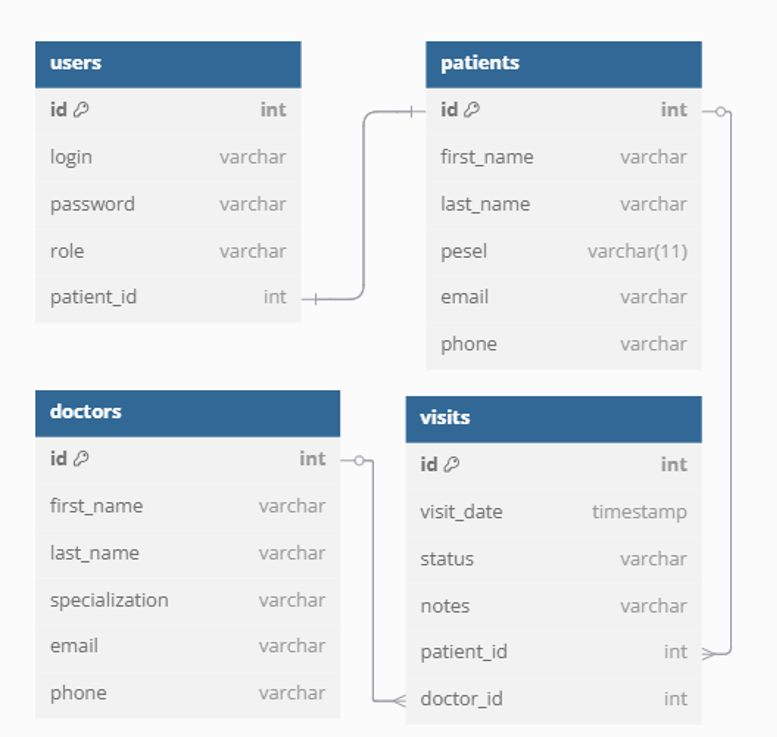
\includegraphics[width=0.85\textwidth]{figures/Diagram_bazy_danych.png}
\caption{Diagram koncepcyjny bazy danych}
\end{figure}

%\clearpage
%\vspace*{\fill}
%\newpage
\section{Diagram klas (dziedziczenie)}
Diagram klas ilustruje hierarchię dziedziczenia między obiektami aplikacji:
\begin{itemize}
    \item Klasa bazowa \textbf{Person} zawiera wspólne dane dla osób: identyfikator, imię, nazwisko, telefon i e-mail.
    \item Klasy \textbf{Doctor} i \textbf{Patient} dziedziczą po klasie \textit{Person}, rozszerzając ją o odpowiednio: \textit{specialization} i \textit{pesel}.
    \item Klasa \textbf{User} przechowuje dane logowania i rolę użytkownika oraz referencję do pacjenta.
    \item Klasa \textbf{Visit} reprezentuje wizytę i zawiera datę, notatki oraz pole \textit{status} przyjmujące jedną z wartości: ZAPLANOWANA, ODBYTA, ANULOWANA.
\end{itemize}
\begin{figure}[H]
\centering
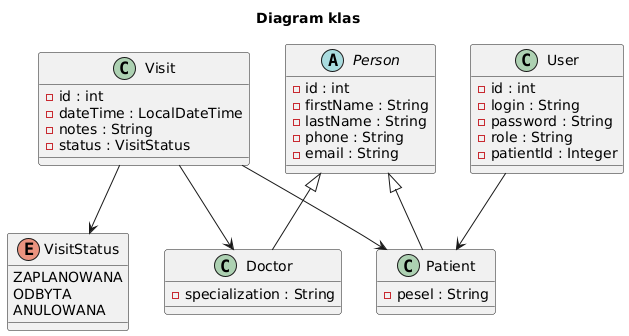
\includegraphics[width=0.85\textwidth]{figures/DiagramKlas.png}
\caption{Diagram klas przedstawiający hierarchię dziedziczenia}
\end{figure}

\section{Opis struktur danych}
System opiera się na czterech głównych encjach:
\begin{itemize}
  \item \textbf{Pacjent} -- dane identyfikacyjne (imię, nazwisko, PESEL, email, telefon),
  \item \textbf{Lekarz} -- imię, nazwisko, email, telefon, specjalizacja,
  \item \textbf{Wizyta} -- powiązanie lekarza z pacjentem, termin, status, notatka,
  \item \textbf{Użytkownik} -- login, hasło, rola (sekretarz lub pacjent), powiązanie z pacjentem (jeśli dotyczy).
\end{itemize}
